\title{Secure unforkable blockchain wallet}
%----------------------------------------------------------------------------------------
%	PACKAGES AND OTHER DOCUMENT CONFIGURATIONS
%----------------------------------------------------------------------------------------

\documentclass[12pt]{article}
\usepackage[english]{babel}
\usepackage[utf8x]{inputenc}
\usepackage{amsmath}
\usepackage{graphicx}
\usepackage[colorinlistoftodos]{todonotes}
\usepackage{float}
\usepackage{csquotes}

\begin{document}

\begin{titlepage}

\newcommand{\HRule}{\rule{\linewidth}{0.5mm}} % Defines a new command for the horizontal lines, change thickness here

\center % Center everything on the page
 
%----------------------------------------------------------------------------------------
%	HEADING SECTIONS
%----------------------------------------------------------------------------------------

\textsc{\LARGE The University of Sydney}\\[1.5cm] % Name of your university/college
\textsc{\Large School of Information Technology}\\[0.5cm] % Major heading such as course name
\textsc{\large Thesis of Master of IT}\\[0.5cm] % Minor heading such as course title

%----------------------------------------------------------------------------------------
%	TITLE SECTION
%----------------------------------------------------------------------------------------

\HRule \\[0.6cm]
{ \huge \bfseries Secure Unforkable Blockchain Wallet}\\[0.4cm] % Title of your document
\HRule \\[1.6cm]
 
%----------------------------------------------------------------------------------------
%	AUTHOR SECTION
%----------------------------------------------------------------------------------------

\begin{minipage}{0.4\textwidth}
\begin{flushleft} \large
\emph{Author:}\\
Lin \textsc{Han} % Your name
\end{flushleft}
\end{minipage}
~
\begin{minipage}{0.4\textwidth}
\begin{flushright} \large
\emph{Supervisor:} \\
Dr. Vincent \textsc{Gramoli} % Supervisor's Name
\end{flushright}
\end{minipage}\\[2cm]

%----------------------------------------------------------------------------------------
%	DATE SECTION
%----------------------------------------------------------------------------------------

{\large \today}\\[2cm] % Date, change the \today to a set date if you want to be precise

%----------------------------------------------------------------------------------------
%	LOGO SECTION
%----------------------------------------------------------------------------------------


\includegraphics{logo.png}\\[1cm] % Include a department/university logo - this will require the graphicx package
 
%----------------------------------------------------------------------------------------

\vfill % Fill the rest of the page with whitespace

\end{titlepage}

\tableofcontents
\vfill

\newpage

% \begin{abstract}
% Your abstract.
% \end{abstract}

\section{Introduction}

% context part, introduction to cryptocurrencies
From the time when Block 0 of Bitcoin blockchain, the Genesis Block, is created at 18:15:05 GMT on January 3rd, 2009, the words ``cryptocurrencies'' and ``Blockchain'' become one of the most popular topics in information technology fields. The ``decentralized'' and ``anonymous'' nature of cryptocurrencies overcomes the weakness of traditional \textit{trust-based} electronic payments who relies heavily on trusted third-party financial institutions. It's cryptography-based nature also make sure its security in some sense. The \textit{cryptographic proof-of-work} of bitcoin enables reliable transaction between two parties directly\cite{nakamoto2008bitcoin}. Through almost 10 years development, cryptocurrencies turns out to be a large family and can be accessed via desktop, laptop, or even mobile devices like smart phones.

% Problem
Though bitcoin gives a practical solution on traditional \textit{double spending} problem in digital currencies, this doesn't mean that it is secure in all aspects. One possible issue is bitcoin blockchain's forkable feature. Actually, other cryptocurrencies allowing forkable chains all suffer from the very same issue. It will become a problem for wallet users if the nodes they are contacting is hijacked. In this sense, unfokable blockchain is proven to overcome this shortcommings\cite{DBLP:journals/corr/CrainGLR17}. To consider in another aspect, another possible solution to secure transaction is to adopt mechanism like \textit{zero knowledge contingent payment} which are released if and only if some knowledge is disclosed by the payee and to do this in a trustless manner where neither the payer or payee can cheat\cite{wiki2011zero}\cite{sasson2014zerocash}. Whilst there are several theoretical discussion and practices in a variety of contexts, this paper will concentrate on how to develop a secure cryptocurrency wallet on the basis of unforkable blockchain and enable secure trades between parties by the help of zero knowledge contingent payments. 

% Contributions
In this project, I intend to contribute in two separated directions: one is to develop a secure mobile client for Red Belly Blockchain - a practice to deploy unforkable blockchain onto modern mobile devices; the other is to explore the way to enable zero knowledge contingent payments within Red Belly Blockchain network. The primary goal of this research is to examine the feasibility of real-life secure application for unforkable blockchain like Red Belly Blockchain.

% Roadmap
In the following report, related works will be given first. Essential concepts and problems will be addressed in this part. After the literature review, the methodologies and proposed contribution is given. After that, detailed report on implementation of secure wallet and zero knowledge contingent payments will be shown. Last but not the least, current outcomes of this project will be discussed. And finally, a conclusion as well as possible improvements and future works will conclude this paper.

% Literature review part
%   this content is comming from assignment 2 Literature review
% TODO: modify it to suit needs of thesis
\section{Literature Review}
\label{sec:Literature Review}

\subsection{Bitcoin}

Bitcoin is the first decentralized digital currency as well as a digital payment system. The whole system is peer-to-peer based, whose transactions are between users directly without participation of intermediary. Transactions are verified by network nodes - known as \textit{mining} - and recorded in a public distributed ledger called \textit{blockchain}.

\subsubsection{Blockchain}

Blockchain is the way how Bitcoin keeps its public ledger within its peer-to-peer network. To some extent, blockchain is a peer-to-peer distributed timestamp server. The ultimate goal of this design is to solve \textit{double-spending} problems and prevent modification of transaction records\cite{nakamoto2008bitcoin}. 

Each full node in the Bitcoin network keeps a full copy of the blockchain, in which all blocks validated by this particular is stored. When several nodes within the network independently arrive at identical blockchains, they are considered to be in \textit{consensus}. As its name suggests, a blockchain is a digital chain of blocks, where a timestamp, a nonce, and a Merkle Tree is stored.  The blocks are chained cryptographically using hash. In detail, each block contains the hash of its previous block ,finally leading to the Genesis Block. Any modification on blocks in the chain would violates all subsequent hashes, which is vital for consistency of the ledger. Figure \ref{fig:blockchain} shows part of a blockchain. 

% blockchain figure here
\begin{figure}
    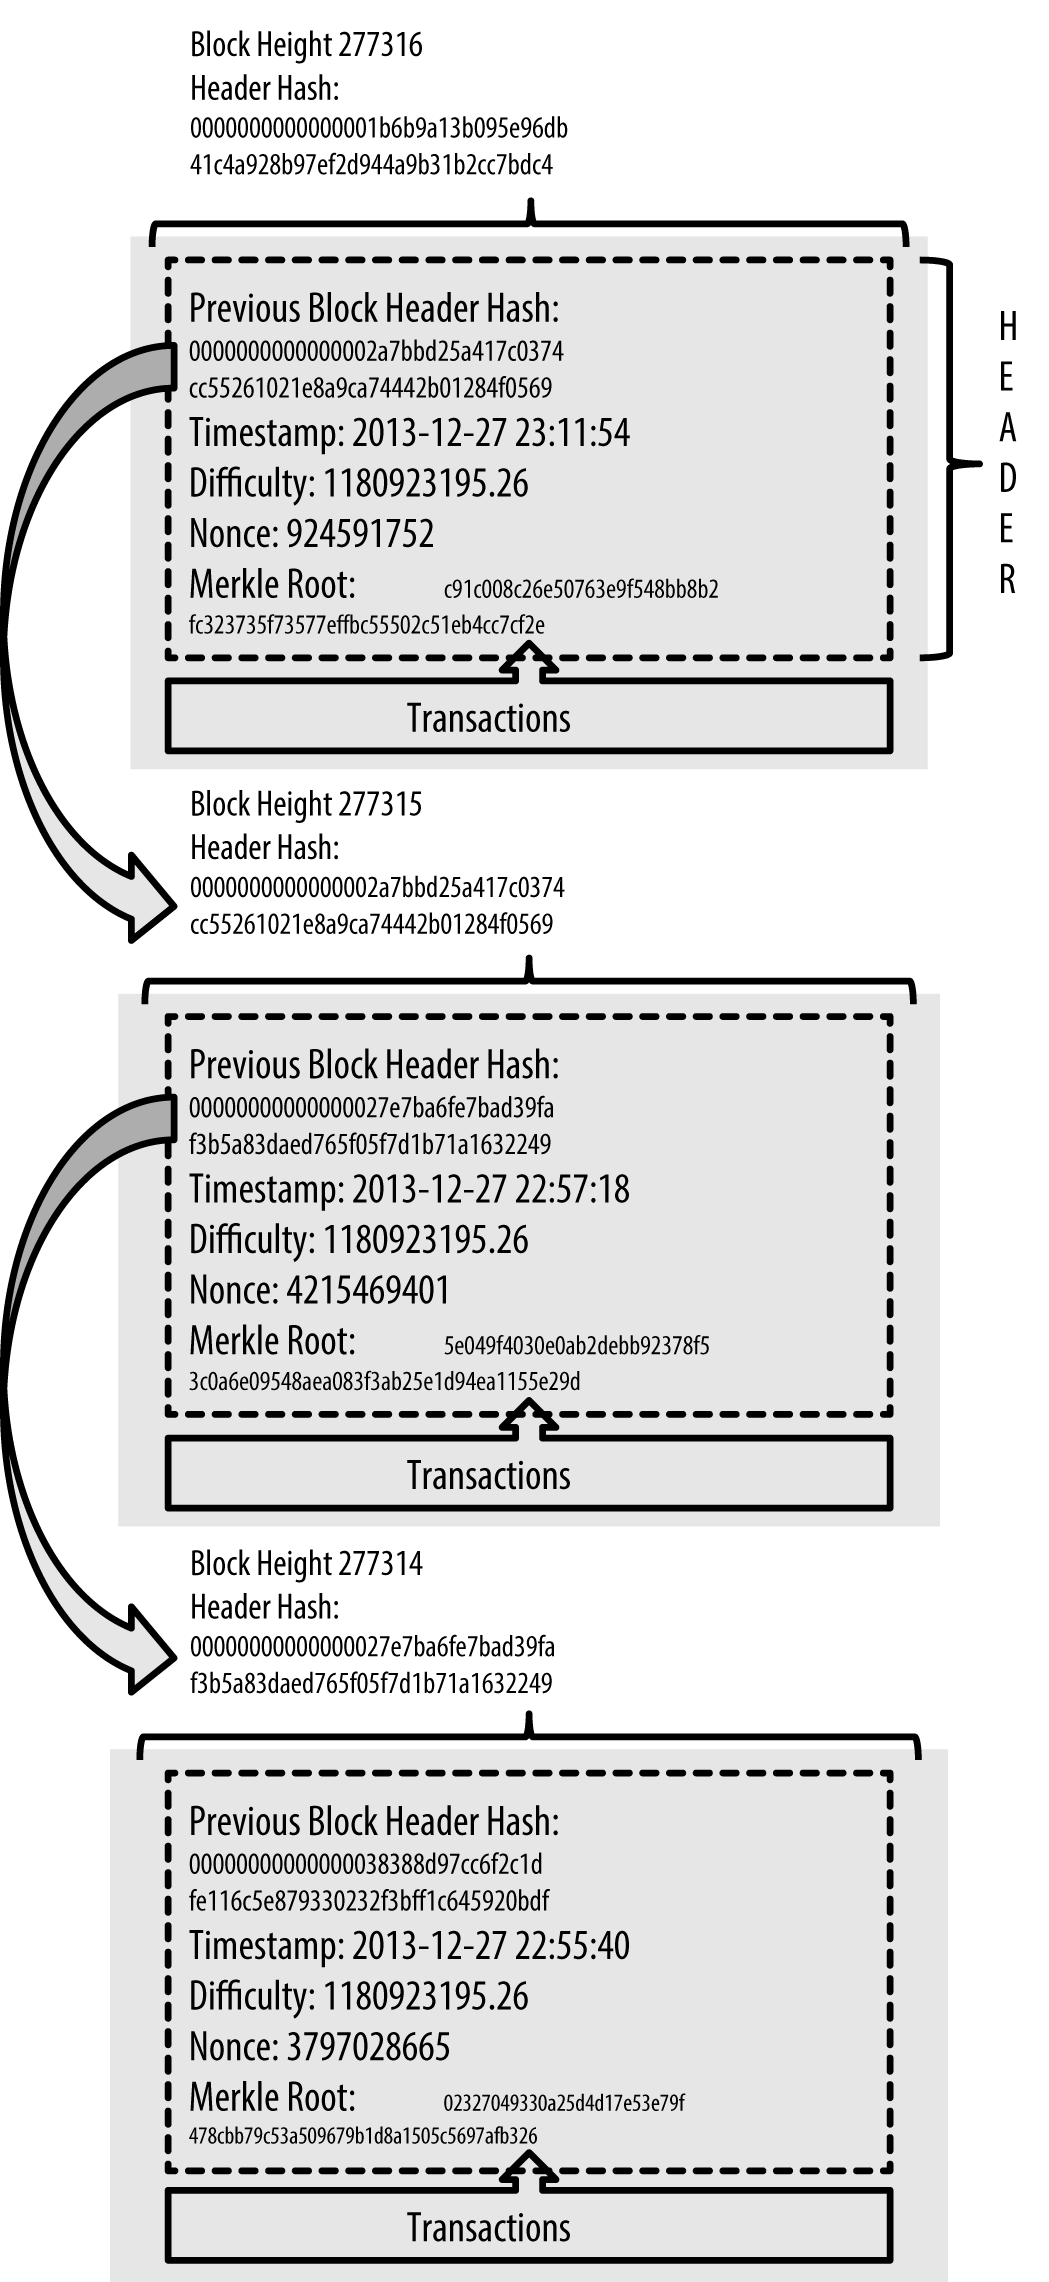
\includegraphics{blockchain.png}
    \caption{Blockchain}
    \label{fig:blockchain}
\end{figure}

However, computing a hash is expensive. This truth enables \textit{proof-of-work} in bitcoin network. 

\subsubsection{Proof of Work}

According to blockchains' feature, a huge amount of computation is required in the generation of each block. Meanwhile, there is a \textit{proof-of-work} mechanism to make the distributed timestamp server work and determine representation in majority decision making. Especially, when there are multiple chains (forks), consensus rules will pick up the longest chain, which contains the most proof of work during its generation\cite{nakamoto2008bitcoin}.

In this way, any malicious changes on previous blocks would violate its following blocks. That is to say, hacker with huge computing power can hijack the blockchain if he can generate the longest chain from the block he hacks. In turn, he has to own more than half of the computing power within the whole blockchain network\cite{NG17}.

\subsubsection{Contracts}

There are distributed contracts in Bitcoin transactions for agreement enforcements, which provides another way to formalize and guarantee agreements rather than traditional court system. Examples include Escrow, Micropayment channels and CoinJoin.

Some of the contracts can be implemented in Bitcoin Script, especially the zero knowledge contingent payments in Bitcoin is achieved with support of bitcoin scripts. However the Red Belly Blockchain doesn't have a robust scripting language like Bitcoin does.

\subsection{Ethereum}

\subsubsection{Previous Work of Bitcoin}

Bitcoin provides a protocol allowing weak implementation of \textit{smart contracts}. However, several limitations exists in Bitcoin's scripting language:

\begin{enumerate}
    \item \textbf{Not Turing-Completeness} - Bitcoin scripts lacks loops.
    \item \textbf{Lack of States} - UTXOs scripts is only for one-off contracts.
    \item \textbf{Blindness of Blockchain} - Bitcoin scripts cannot access blockchain data.
    \item \textbf{Blindness of Value} - Bitcoin either consumes the entire UTXO or none of it
\end{enumerate}

\subsubsection{Rationale}

Ethereum implements a blockchain with Turing-complete scripts, states, value awareness and blockchain awareness, which enables development of smart contracts, and even new protocols\cite{wood2014ethereum}.

\subsection{Balance Attack}
\label{sec:Balance Attack}

As the previous review mentioning, to attack a blockchain, or specifically to rewrite the content of a block, the hacker should have more than half of the computing power of the whole blockchain network which is almost unfeasible in real world. In particular, by delaying the propagation of blocks in Bitcoin system, the hacker can in result delay the growth of the longest branch of the system. In other word, he can then hijack the blockchain even without a large amount of computing power. Ethereums' ``Blockchain 2.0'' somehow fixes this problem, but there is still other possible method against forked blockchain. One practice is the \textbf{Balance Attack} \cite{Gra16}\cite{NG17}\cite{NG16}against \textit{proof-of-work} blockchain systems.

To achieve a balance attack within the blockchain network, the attacker should divide the network into subgroups of similar mining power by cutting off their communications. During this down time, the attacker issues transaction in the \textit{transaction group}, and mine blocks in the \textit{block group} simultaneously. This action only ends when it comes to the point where the tree of the block subgroup outweighs the tree of the transaction group, which is with high possibility. The balance, in result, can leverage the \textit{GHOST} protocol that accounts for sibling or uncle blocks to determine on a chain of blocks. This strategy allows the attacker to mine a branch regardless of the rest of the network so that he can influence the branch determination process while merging\cite{NG17}. The process is as shown in Figure \ref{fig:balance_attack}.

\begin{figure}
    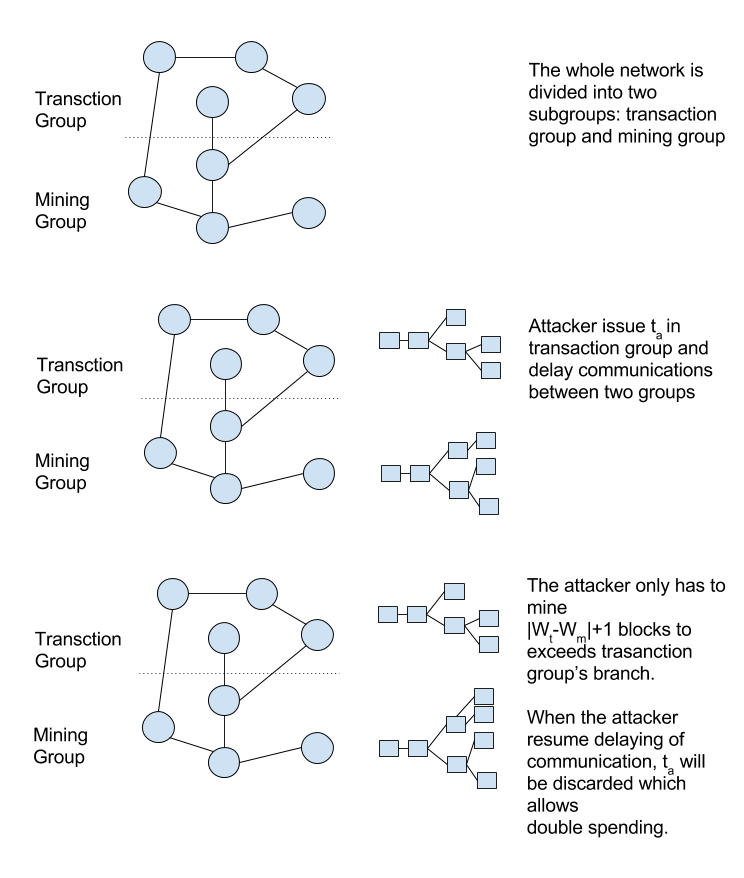
\includegraphics{balance_attack.png}
    \caption{Balance Attack}
    \label{fig:balance_attack}
\end{figure}

\subsection{Unforkable Blockchain}
\label{sec:Unforkable Blockchain}

\subsubsection{Byzantine Consensus Problem}

The \textit{Byzantine Consensus Problem} refers to the \textit{Byzantine General's Problem} proposed by Leslie Lamport, Robert Shostak and Marshall Pease in 1982. The problem is complicated by the presence of traitorous generals who may not only cast a vote for a suboptimal strategy, they may do so selectively. All the votes and results are simplified to attack or retreat. The problem is complicated further by the generals being physically separated and having to send their votes via messengers who may fail to deliver votes or may forge false votes\cite{lamport1982byzantine}.

In computer science area, typically computers or participants in network are mapped to generals and links between them are mapped to messengers.

\subsubsection{Traditional Blockchain Byzantine Consensus Problem}

The \textit{proof-of-work} of Bitcoin blockchain is the primary solution to \textit{Byzantine Consensus Problem}. 

In detail, a model of Bitcoin network can be built upon the classic Byzantine Consensus Problem. The distributed system is the alliance of generals, in which the upper bounds on the delay of communicating and decision-making is unknown. 

However, regarding to our previous discussion on \textit{Balance Attack}, attackers can still disrupt the consensus system to beat the Bitcoin Byzantine Consensus\cite{gramoli2017blockchain}. Because there is no guarantee that the decided value is proposed by a valid process.

\subsubsection{Democratic Byzantine Consensus}

Democratic Byzantine Fault Tolerance is a system specially tailored for consortium blockchains based on \textit{Binary Byzantine Consensus}. In \textit{Binary Byzantine Consensus}\cite{mostefaoui2015signature}, each trusted participant issue proposal with either 0 or 1 and decides that the final agreement such that:

\begin{enumerate}
    \item No pair of trusted participants have different decision.
    \item Every trusted participant decides
    \item If all correct participant propose the the same value, then no other value can be deiced
\end{enumerate}

In safe Democratic Byzantine Fault Tolerance\cite{DBLP:journals/corr/CrainGLR17}, a mechanism called binary broadcast for binary Byzantine Consensus system is adopted. To conclude, there are four aspects that is strictly followed within DBFT:

\begin{enumerate}
    \item \textbf{Binary Value Obligation} - if t+1 correct BV-broadcats $v$, then $v$ is eventually added to the set binary values of all correct process.
    \item \textbf{Binary Value Justification} - if $p_i$ is correct and and $v$ in $binary-values_i$ then $v$ was broadcasted by a correct process.
    \item \textbf{Binary Value Uniformity} - if $v$ is added to $binary-value_i$ of correct $p_i$, then eventually $v$ will be in $binary-value_j$ for all correct $p_j$.
    \item \textbf{Binary Value Termination} - eventually $binary-value$ of correct $p_i$ is not empty. 
\end{enumerate}

\subsection{The Red Belly Blockchain}

Red Belly Blockchain is new blockchain relying on the Democratic BFT. The \textit{Genesis Block} of this blockchain contains the initial information as well as a list of n participants. All accesses of external nodes requires these participants as the middleware. In this case, a transaction is regarded as committed if $t+1$ participating nodes agreed so it can be written into next block.

The performance of this new blockchain is quite good. It can achieve more than 400 transactions per second and with great scalability up to 90 server nodes.

\subsection{Zero Knowledge Contingent Payment}
\label{sec:Zero Knowledge Contingent Payment}

\subsubsection{Bitcoin ZKCP}

Zero Knowledge Contingent Payment in Bitcoin is first proposed by Gregory Maxwell in 2011 on Bitcoin Wiki\cite{maxwell5zero}. The basic process can be illustrated by an example\cite{campanelli2017zero}:

\begin{displayquote}
    Alice is a fan of Sudoku puzzle. However, there is a puzzle that she is trying days but in vain. She gives up and broadcasts a message within a fan group proclaiming that ``I will pay whoever solves this puzzle.'' Bob see the broadcast, solves it, and want to sell the result to Alice. The problem is either Alice or Bob is willing to be the first person to give out what they have.

    To solve this dilemma, Alice and Bob goes for a Bitcoin, which allows one to issue a transaction and also specify the conditions to be met in order to claim the transaction. In this case, Alice propose a payment transaction to blockchain that includes encoded Sudoku puzzle and the rules. Whoever solves the puzzle is able to get the fund.

    Using the Bitcoin ZKCP protocol, Bob knows a solution $s$ and encrypts the solution using a key $k$ such that $Enc_k(s)=c$ and he computes $y$ such that $SHA256(k)=y$. He then send the key $k$ and $c$ to Alice together with a zero knowledge proof that $c$ is an encryption of $s$ under the key $k$ and  that $SHA256(k)=y$. Once Alice has verified the proof, she creates a transaction to the blockchain that pays Bob $n$ bitcoins, and says that Bob can only claim the coins if he provides the value $k'$ such that $SHA256(k')=y$. Bob then published $k$ and claims the fund. In this way, Alice learns $k$ can decrypt c so that she knows the solution $s$
\end{displayquote}

Specifically in Blockchain, the ZKCP protocol now has several practices rather than theory. One is ZK-SNARK protocols allowing for the practical implementation of the necessary proofs\cite{kalai2006succinct}\cite{ben2015secure}\cite{ecc2011}.

\subsubsection{Zero Knowledge Contingent Payment without Scripts}

However, all implemented ZKCP protocols now are based on scripting language in traditional forkable blockchain\cite{Banasik2016}. Besides, there is no convincing data of its performance on modern mobile devices\cite{doi:10.1080/00207160.2014.933816}.

\section{Motivation}

From the above review of cryptocurrencies and blockchain contexts, one can conclude that the blockchain technology adopted by cryptocurrencies nowadays has potential risks regarding to its forkable nature. This also influence the usage of current cryptocurrency wallet - there is no guarantee that the proposed transaction (or retrieved balance) from wallet is securely handled by the server if it contacts only one single machine.

Hence, the motivation of this research comes from this gap. The aim of this research is to develop a wallet making both transaction proposing and balance retrieving reliable and correct. During the first part of this research, a secure wallet will be developed, perfoming in a Red Belly Blockchain way to avoid possible attacks targeting at fork chains. The Zero Knowledge Contingent Proof will try to add another guarantee so that either party within a transaction cannot cheat for its own benefits.

\section{Methodologies and Proposed Contributions}

\subsection{Previous Work}

This research is on the basis of Red Belly Blockchain which is an unforkable blockchain running \textit{Democratic Byzantine Fault Tolerance}. The development of secure wallet is build upon the implementation of Red Belly Blockchain.

In Red Belly Blockchain, all nodes are communicated through TCP+SSL. Nodes in this blockchain consists of nodes running Byzantine Consensus Algorithms - the \textit{participants}, and external nodes communicating with the \textit{participants}. A transaction or balance of an account can only be considered correct if more than one thirds of the \textit{participants} agreed as required by DBFT.

\subsection{Proposed Contributions}

To develop a secure wallet, a secure protocol between server and clients is required. In this project, TCP and SSL is chosen to be the techniques for communications. I intent to implement \textit{remote procedure call} for Red Belly Blockchain nodes first so that further functions can be achieved on client side. 

Regarding to the client, I intend to implement secure wallet basic balance and transaction request functions complying with the same DBFT algorithm as Red Belly Blockchain nodes. In this sense, users of wallet can make sure that the balance and transaction are correctly obtained or proposed respectively.

In addition to server enhancement and secure wallet development, the pursuit of security also motivated this research to develop a Zero Knowledge Contingent Payments model for RBBC so that no party can cheats within such a `contract'. The ZKCP implementation in RBBC is not like the one in Bitcoin who has scripts supporting this function while RBBC doesn't have.

\subsection{Methodologies}

The ultimate goal of this research is to develop a wallet that enables secure balance retrieving, transaction proposing, as well as trading. This would require design and development in both server side and client side.

The first part of this project is to add secure \textit{remote procedure call} to Red Belly Blockchain. The \textit{RPC} protocol should be through TCP and SSL. Once the \textit{RPC} server is ready, Java and Android client could be developed based on it. After the client is developed, benchmarks on speed of balance retrieving and transaction proposing is required. And at the end of the above, I'll explore to develop a model to integrate \textit{Zero Knowledge Contingent Payments} into the application. 

\section{Secure Wallet}

In this report, secure wallet refers to two parts: the Red Belly Blockchain wallet and the Zero Knowledge Contingent Payments Model. This paper will explain the design and implementation of secure wallet in detail respectively.

\subsection{Red Belly Blockchain Wallet}

\subsubsection{Preliminaries}

\subsubsection{Functions of Red Belly Blockchain Wallet}

\subsubsection{Design of Red Belly Blockchain Wallet}

\subsubsection{Red Belly Blockchain Compatibility}

\subsubsection{implementation of Red Belly Blockchain Wallet}


\subsection{Zero Knowledge Contingent Payments}


% TODO: modify conclusion
\section{Conclusion}

In this literature review, we can see that unforkable blockchain has a more reliable security guarantee compared to traditional forkable blockchain used in mainstream cryptocurrencies. The need to deploy unforkable blockchain and implement ZKCP-enable protocols onto mobile devices is evident through the literatures to fulfill the gaps between the theoretical discussion and real life application. Deploying ZKCP-enbale unforkable blockchains onto mobile devices will benefit both authorities seeking reliable blockchain solutions and users having trust problems with third-parties.

\newpage
\bibliography{bibliography.bib}
\bibliographystyle{plain}

\end{document}
